%%%%%%%%%%%%%%%%%%%%%%%%%%%%%%%%%%%%%%%
% Wenneker Resume/CV
% LaTeX Template
% Version 1.1 (19/6/2016)
%
% This template has been downloaded from:
% http://www.LaTeXTemplates.com
%
% Original author:
% Frits Wenneker (http://www.howtotex.com) with extensive modifications by 
% Vel (vel@LaTeXTemplates.com)
%
% License:
% CC BY-NC-SA 3.0 (http://creativecommons.org/licenses/by-nc-sa/3.0/
%
%%%%%%%%%%%%%%%%%%%%%%%%%%%%%%%%%%%%%%

%----------------------------------------------------------------------------------------
%	PACKAGES AND OTHER DOCUMENT CONFIGURATIONS
%----------------------------------------------------------------------------------------

\documentclass[a4paper,12pt]{memoir} % Font and paper size

%%%%%%%%%%%%%%%%%%%%%%%%%%%%%%%%%%%%%%%%%
% Wenneker Resume/CV
% Structure Specification File
% Version 1.1 (19/6/2016)
%
% This file has been downloaded from:
% http://www.LaTeXTemplates.com
%
% Original author:
% Frits Wenneker (http://www.howtotex.com) with extensive modifications by 
% Vel (vel@latextemplates.com)
%
% License:
% CC BY-NC-SA 3.0 (http://creativecommons.org/licenses/by-nc-sa/3.0/)
%
%%%%%%%%%%%%%%%%%%%%%%%%%%%%%%%%%%%%%%%%%

%----------------------------------------------------------------------------------------
%	PACKAGES AND OTHER DOCUMENT CONFIGURATIONS
%----------------------------------------------------------------------------------------

\usepackage{XCharter} % Use the Bitstream Charter font
\usepackage[utf8]{inputenc} % Required for inputting international characters
\usepackage[T1]{fontenc} % Output font encoding for international characters

\usepackage[top=1cm,left=1cm,right=1cm,bottom=1cm]{geometry} % Modify margins

\usepackage{graphicx} % Required for figures

\usepackage{flowfram} % Required for the multi-column layout

\usepackage{url} % URLs

\usepackage[usenames,dvipsnames]{xcolor} % Required for custom colours

\usepackage{tikz} % Required for the horizontal rule

\usepackage{enumitem} % Required for modifying lists
\setlist{noitemsep,nolistsep} % Remove spacing within and around lists

\setlength{\columnsep}{\baselineskip} % Set the spacing between columns

% Define the left frame (sidebar)
\newflowframe{0.2\textwidth}{\textheight}{0pt}{0pt}[left]
\newlength{\LeftMainSep}
\setlength{\LeftMainSep}{0.2\textwidth}
\addtolength{\LeftMainSep}{1\columnsep}
 
% Small static frame for the vertical line
\newstaticframe{1.5pt}{\textheight}{\LeftMainSep}{0pt}
 
% Content of the static frame with the vertical line
\begin{staticcontents}{1}
\hfill
\tikz{\draw[loosely dotted,color=RoyalBlue,line width=1.5pt,yshift=0](0,0) -- (0,\textheight);}
\hfill\mbox{}
\end{staticcontents}
 
% Define the right frame (main body)
\addtolength{\LeftMainSep}{1.5pt}
\addtolength{\LeftMainSep}{1\columnsep}
\newflowframe{0.7\textwidth}{\textheight}{\LeftMainSep}{0pt}[main01]

\pagestyle{empty} % Disable all page numbering

\setlength{\parindent}{0pt} % Stop paragraph indentation

%----------------------------------------------------------------------------------------
%	NEW COMMANDS
%----------------------------------------------------------------------------------------

\newcommand{\userinformation}[1]{\renewcommand{\userinformation}{#1}} % Define a new command for the CV user's information that goes into the left column

\newcommand{\cvheading}[1]{{\Huge\bfseries\color{RoyalBlue} #1} \par\vspace{.6\baselineskip}} % New command for the CV heading
\newcommand{\cvsubheading}[1]{{\Large\bfseries #1} \bigbreak} % New command for the CV subheading

\newcommand{\Sep}{\vspace{1em}} % New command for the spacing between headings
\newcommand{\SmallSep}{\vspace{0.5em}} % New command for the spacing within headings

\newcommand{\aboutme}[2]{ % New command for the about me section
\textbf{\color{RoyalBlue} #1}~~#2\par\Sep
}
	
\newcommand{\CVSection}[1]{ % New command for the headings within sections
{\Large\textbf{#1}}\par
\SmallSep % Used for spacing
}

\newcommand{\CVItem}[2]{ % New command for the item descriptions
\textbf{\color{RoyalBlue} #1}\par
#2
\SmallSep % Used for spacing
}

\newcommand{\bluebullet}{\textcolor{RoyalBlue}{$\circ$}~~} % New command for the blue bullets
 % Include the file specifying document layout and packages

%----------------------------------------------------------------------------------------
%	NAME AND CONTACT INFORMATION 
%----------------------------------------------------------------------------------------

\userinformation{ % Set the content that goes into the sidebar of each page
\begin{flushright}
% Comment out this figure block if you don't want a photo
% \includegraphics[width=0.6\columnwidth]{photo.png}\\[\baselineskip] % Your photo
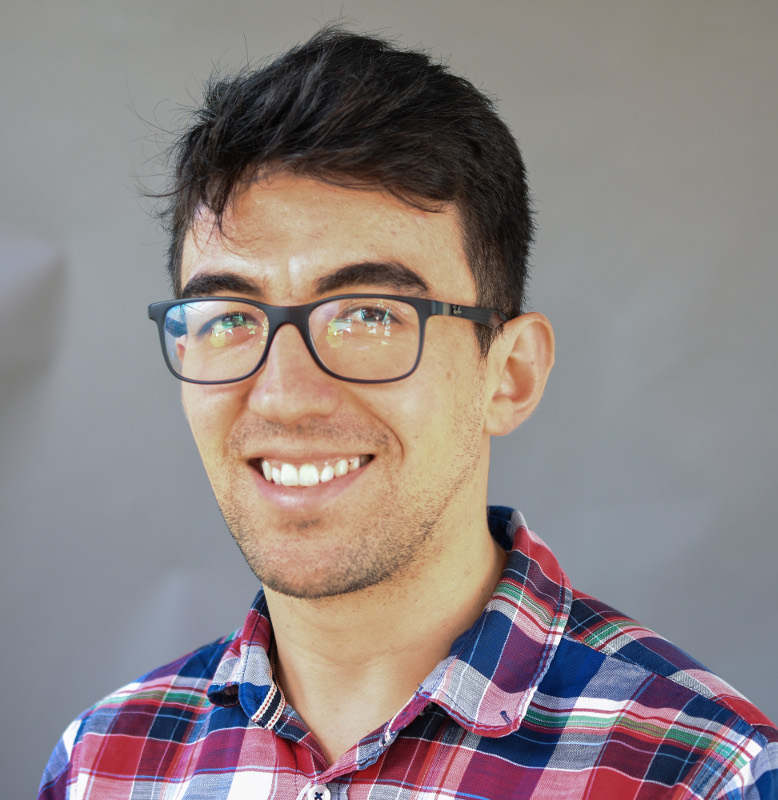
\includegraphics[width=0.7\columnwidth]{PhotoLinkedinshort.jpg}
\small % Smaller font size
Nikolay Prieto \\ % Your name
\scriptsize{\url{enprietop@unal.edu.co}} \\ % Your email address
% \url{www.johnsmith.com} \\ % Your URL
+57 (300) 350 1177 \\ % Your phone number
\Sep % Some whitespace
\textbf{Dirección} \\
Calle 12 # 3-05 \\ % Address 1
La Calera, Cundinamarca \\ % Address 2
Colombia \\ % Address 3
\vfill % Whitespace under this block to push it up under the photo
\end{flushright}
}

%----------------------------------------------------------------------------------------

\begin{document}

\userinformation % Print your information in the left column

\framebreak % End of the first column

%----------------------------------------------------------------------------------------
%	HEADING
%----------------------------------------------------------------------------------------

\cvheading{Nikolay Prieto} % Large heading - your name

\cvsubheading{Ingeniero Mecatrónico} % Subheading - your occupation/specialization

%----------------------------------------------------------------------------------------
%	ABOUT ME
%----------------------------------------------------------------------------------------

\aboutme{Acerca de mí}{Candidato a doctor en ingeniería mecánica y mecatrónica, enfocado al análisis de datos en la marcha humana y al diseño mecánico óptimo de dispositivos biomecánicos. Cuento con conocimiento y experiencia industrial en gestión de proyectos, investigación y docencia universitaria. Poseo excelentes habilidades en programación, automatización y modelado físico computacional. Por otro lado, en cuanto a las habilidades blandas considero que cuento con las siguientes: excelente comunicación, liderazgo, aprendizaje continuo, autónomo, persistente y orientado hacia objetivos, aplicando pensamiento ingenieril a la solución de problemas de nuestro entorno. Actualmente quisiera dedicarme a la aplicación de investigación a nivel industrial y/o docencia universitaria.}

%----------------------------------------------------------------------------------------
%	EDUCATION
%----------------------------------------------------------------------------------------

\CVSection{Educación}

%------------------------------------------------

\CVItem{2014 - , Universidad Nacional de Colombia}{\textbf{Doctorado en Ingeniería.} \\
\textbf{título de tesis:} \textit{Passive Dynamic System for Energy Returning on Transtibial Prosthesis.} \\
\textbf{Promedio General:} 4.4/5.0 \\
\textbf{Módulos Incluidos:}
\begin{itemize}
    \item Ingeniería Biomecánica
    \item Procesos Avanzados de Manufactura
    \item Aplicaciones Avanzadas con Elementos Fínitos
    \item Vizualización de Datos y Aprendizaje de Máquina.
    \item Optimización Topológica.
    \item Optimización Bio-inspirada.
\end{itemize}}
%------------------------------------------------
\CVItem{2011 - 2014, Universidad Militar de Colombia}{M.Engr. en Mecatrónica} \\
\textbf{Título de la tesis:} \textit{Diseño, simulación y fabricación de una prótesis de alto impacto para amputados de miembro inferior.} \\
\textbf{Promedio General:} 4.5/5.0 \\
\textbf{Módulos Incluidos:}
\begin{itemize}
    \item Estrategias Avanzadas de Control. 
    \item Análisis de sistemas no lineales.
    \item Sistemas Embebidos.
    \item Materiales y Manufactura.
    \item Análisis de Elementos Finitos.
\end{itemize}

\CVItem{2004 - 2009, Universidad de San Buenaventura, Bogotá}{Ingeniero Mecatrónico}
%------------------------------------------------

\Sep % Extra whitespace after the end of a major section

%----------------------------------------------------------------------------------------
%	EXPERIENCE
%----------------------------------------------------------------------------------------

\CVSection{Experiencia}

%------------------------------------------------
\CVItem{Feb. 2019 - Presente, \textit{Profesor Asociado}, Universidad ECCI}{
Actividades Realizadas:
\begin{itemize}
    \item Docencia Universitaria (Automatización - 8 h/sem)
    \item Docencia Universitaria (Expresión gráfica - 16 h/sem)
    \item Funciones sustantivas relacionadas a la investigación.
\end{itemize}
}

%------------------------------------------------
% ----------------------------
%	NEW PAGE DELIMITER
%	Place this block wherever you would like the content of your CV to go onto the next page
%----------------------------------------------------------------------------------------

\clearpage % Start a new page

\userinformation % Print your information in the left column

\framebreak % End of the first column
%------------------------------------------------------------

\CVItem{Jun. 2018 - Dic. 2018, \textit{Asistente de Investigación}, Indiana University Purdue University-Indianapolis (IUPUI)}{
Actividades Realizadas:
\begin{itemize}
    \item Diseño de dispositivos médicos.
    \item Estructurar Algoritmos de Optimización Topológica.
    \item Manufactura Aditiva.
    \item Dieño CAD y Simulaciones no lineales en LS-DYNA.
    \item Inyección de plásticos.
\end{itemize}
}

\CVItem{Feb. 2015 - Jun. 2018, \textit{Profesor auxiliar}, Universidad Nacional de Colombia}{\textbf{Materia Impartida:}: Taller de Proyectos Interdisciplinarios. \\
Materia perteneciente a la facultad de ingeniería, en el cual ponen en práctica los conocimientos en gestión de proyectos y el saber de cada ingeniería.}



\CVItem{Feb. 2009 - Sep. 2014, \textit{Coordinador de proyectos División de Investigación y Desarrollo}, Industria Militar de Colombia (INDUMIL)}{Gestión de proyectos de la parte técnica y administrativa enfocada en investigación y desarrollo tecnológico para el sector de la defensa. }
%----------------------------------------------------------------------------------------
%	COMMUNICATION SKILLS
%----------------------------------------------------------------------------------------

\CVSection{Habilidades Comunicativas.}

%------------------------------------------------
\CVItem{2014, \textit{Congreso}, Congreso Nacional de Fisioterapia ASCOFI.}{\textbf{Título:} Lower Limb Prosthesis: A review }

\CVItem{2013, \textit{Presentación Oral}, Solidworks World 2013, Orlando, Florida, USA.}{\textbf{Talk title:} Anti-explosive Tele-operated Robot and Lower Limb Prosthesis.}

\CVItem{2013, \textit{Presentación Oral}, ESSS-CAE Industry Aerospace and Defense congress}{\textbf{Talk title:} Determination of internal pressure, velocity and recoil in water jet cannons with AutoDYN. Bogotá}

\CVItem{2013, \textit{Article}, Revista Ciencia y Tecnología del Ejército}{\textbf{Talk title:} Determination of internal pressure, velocity and recoil in water
jet cannons with AutoDYN.}
%------------------------------------------------

\Sep % Extra whitespace after the end of a major section

%----------------------------------------------------------------------------------------
%	SKILLS
%----------------------------------------------------------------------------------------

\CVSection{Habilidades en Desarrollo de Software.}

%------------------------------------------------

\CVItem{Programación}
{\begin{tabular}{p{0.2\textwidth} p{0.2\textwidth} p{0.2\textwidth}}
\bluebullet Python &  \bluebullet Matlab & \bluebullet Shell\\
\end{tabular}}

%------------------------------------------------

\CVItem{Manejo de software comercial}
{\begin{tabular}{p{0.2\textwidth} p{0.2\textwidth} p{0.2\textwidth}}
 \bluebullet Windows &  \bluebullet Linux & \bluebullet LS-DYNA\\
 \bluebullet ANSYS &  \bluebullet Inventor & \bluebullet AutoCAD\\
 \bluebullet ALTIUM Designer & \\
\end{tabular}}

%-----------------------------------

\CVItem{Open Source}

{\begin{tabular}{p{0.2\textwidth} p{0.2\textwidth} p{0.2\textwidth}}
\bluebullet \LaTeX &  \bluebullet Opensim & \bluebullet Octave\\
\bluebullet FeBio &  \bluebullet Gmsh & \bluebullet G-code\\
\end{tabular}}
%------------------------------------------------

\Sep % Extra whitespace after the end of a major section
% ----------------------------
%	NEW PAGE DELIMITER
%	Place this block wherever you would like the content of your CV to go onto the next page
%----------------------------------------------------------------------------------------

\clearpage % Start a new page

\userinformation % Print your information in the left column

\framebreak % End of the first column
%------------------------------------------------------------
%	AWARDS
%----------------------------------------------------------------------------------------

\CVSection{Reconocimientos}

%------------------------------------------------

\CVItem{2015, \textit{Exención Derechos Académicos}, Universidad Nacional de Colombia}{Mejor promedio durante el semestre 2014-II.}

\CVItem{2014, \textit{Crédito-beca COLCIENCIAS}, COLFUTURO}{Patrocinio matrícula y sostenimiento durante programa académico del doctorado.}


\CVItem{2011, \textit{Beca Maestría}, Industria Militar de Colombia}{Patrocinio completo del programa.}
%------------------------------------------------

\Sep % Extra whitespace after the end of a major section
%----------------------------------------------------------------------------------------
%	LANGUAGES
%----------------------------------------------------------------------------------------
\CVSection{Idiomas.}
\begin{itemize}
    \item Español (Nativo)
    \item Inglés (547 TOEFL ITP)
\end{itemize}

\Sep

%----------------------------------------------------------------------------------------
%	INTERESTS
%----------------------------------------------------------------------------------------

\CVSection{Intereses}

%------------------------------------------------

\CVItem{Profesionales}{Educación, Investigación, Programación, Biomecánica, Ciencias de la computación, Manufactura Aditiva, FEA.}

%------------------------------------------------

\CVItem{Personales}{Volleyball, Correr, Cocinar, Viajar.}

%------------------------------------------------

\Sep % Extra whitespace after the end of a major section

%----------------------------------------------------------------------------------------

\end{document}
